
\documentclass{article}
\usepackage{graphicx}
\usepackage[margin=1in]{geometry}
\title{Fiber Amplifier and Diamond Raman Laser Standard Operating Procedure}
\author{Jeremy W. Jarrett \and Shaun Engelmann}
\date{Last Updated: 5/20/2021}

\begin{document}
\maketitle
\tableofcontents
\newpage

\section{Optical Layouts}
\begin{figure}[ht]
  \centering
  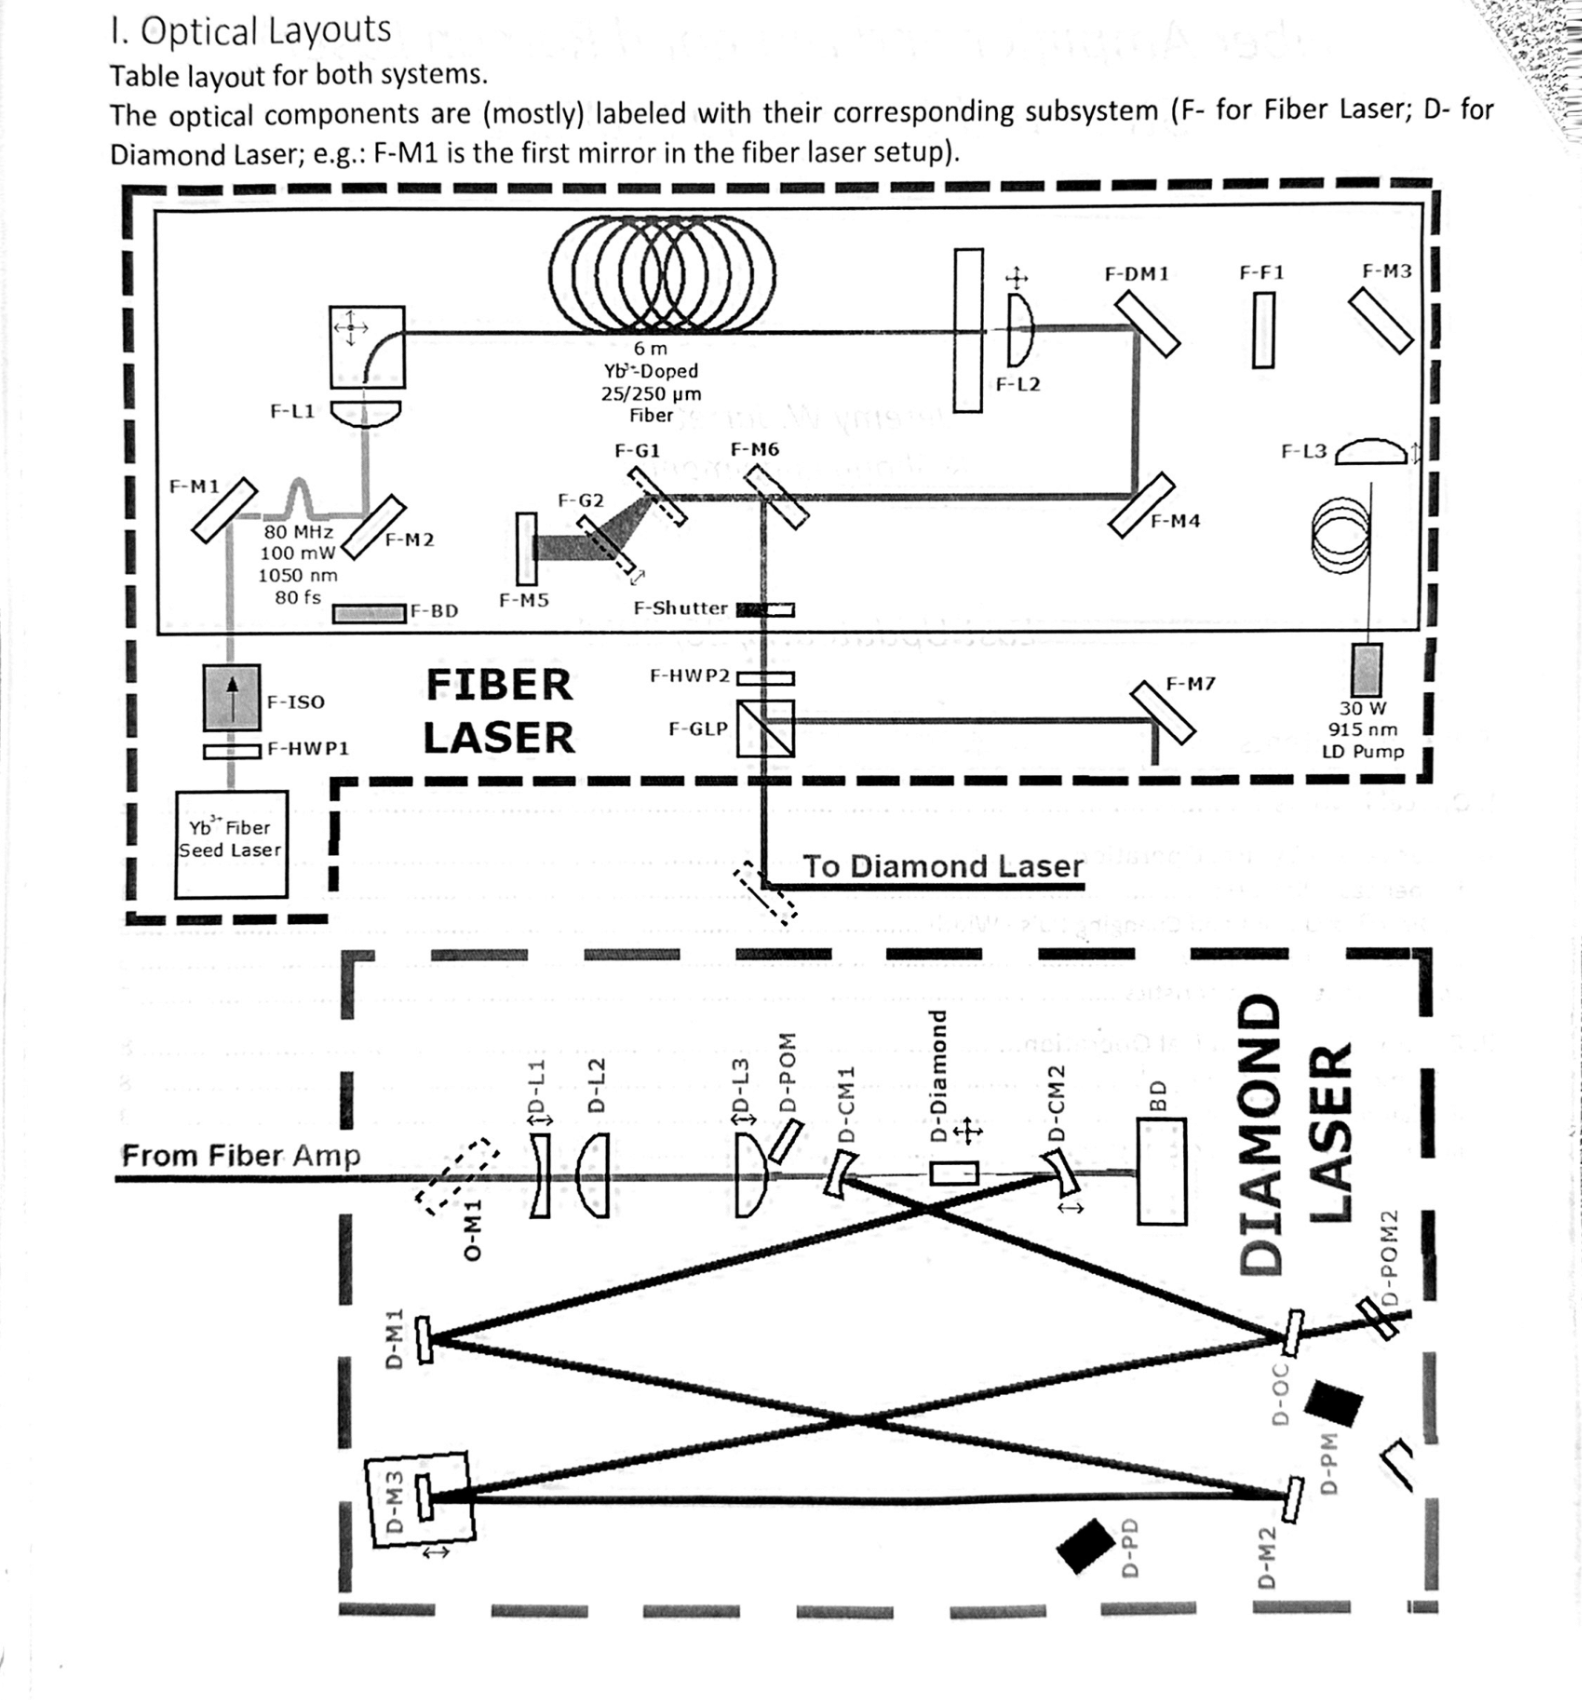
\includegraphics[width=0.9\linewidth]{optical_layout.png}
  \caption{Optical layout diagram.}
\end{figure}

\section{Fiber Laser -- Typical Operation}

\subsection{Fiber Laser Start Up}
\begin{enumerate}
  \item Turn key to ``on'' on the fiber laser controller box. Lights will flash as the oscillator begins its start-up procedure.
  \item While the oscillator warms up, turn on the pump temperature controller (I/O switch) and start the Arroyo control software on the computer.
  \item Select ``Connect'' and then set the output to ``On'' in the Arroyo software.
    \begin{itemize}
      \item The temperature should be set to 25\,$^\circ$C.
      \item \textit{Make sure that the fan on the TEC is spinning. If not, the diode will overheat at high output power.}
    \end{itemize}
  \item Turn on the pump power controller.
  \item Once the oscillator has finished its start-up sequence, press the red button on the controller box to let the seed laser out.
    \begin{itemize}
      \item The red button will illuminate once pressed.
      \item If everything is working correctly with the oscillator, there should be a pulse train visible on the oscilloscope.
    \end{itemize}
  \item Position the high-power meter between F-Shutter and F-HWP2.
  \item Open (``enable'') the shutter to make sure the output will reach the power meter.
  \item Engage the pump diode (press ``Output'' button; blue LED should light) and slowly ramp up the pump current to as high as 8000\,mA.
    \begin{itemize}
      \item Recommended readings:
      \begin{itemize}
        \item ~0.2\,W at 2000\,mA
        \item ~2.3\,W at 4000\,mA
        \item ~4.8\,W at 6000\,mA
        \item ~7.5\,W at 8000\,mA
      \end{itemize}
      \item \textbf{Do not raise the pump current if power seems low at previous checkpoints!}
    \end{itemize}
  \item Let the laser warm up for $\sim$10\,minutes.
  \item Shutter the laser with F-Shutter, place meter in one GLP path, deactivate shutter, and rotate F-HWP2 to adjust power.
\end{enumerate}

\subsection{Directing Output and Changing Pulse Width}
\begin{enumerate}
  \item \textbf{Directing Output:} The output can be split into two paths via F-GLP (imaging vs.\ diamond pump). For diamond, use F-HWP2. If only imaging, block the diamond path.
  \item \textbf{Changing Pulse Width:} Controlled by grating pair F-G1 \& F-G2. Positions for shortest pulse at focus:
    \begin{itemize}
      \item 6.625 @ 4000\,mA
      \item 4.75  @ 6000\,mA
      \item 2.5   @ 8000\,mA (use 2.75 for diamond at 8000\,mA)
    \end{itemize}
\end{enumerate}

\subsection{Fiber Laser Shut Down}
\begin{enumerate}
  \item Close shutter (press ``enable'').
  \item Ramp down pump current to 1000\,mA (250\,mA steps).
  \item Wait 1--2\,minutes.
  \item Turn off pump controller (I/O switch).
  \item Turn off seed oscillator (key to ``off'').
  \item Wait 10--15\,minutes for cooling.
  \item In Arroyo, turn off cooler output then ``Disconnect''.
  \item Turn off laser cooler (I/O switch).
\end{enumerate}

\subsection{Fiber Laser Characteristics}
\begin{figure}[ht]
  \centering
  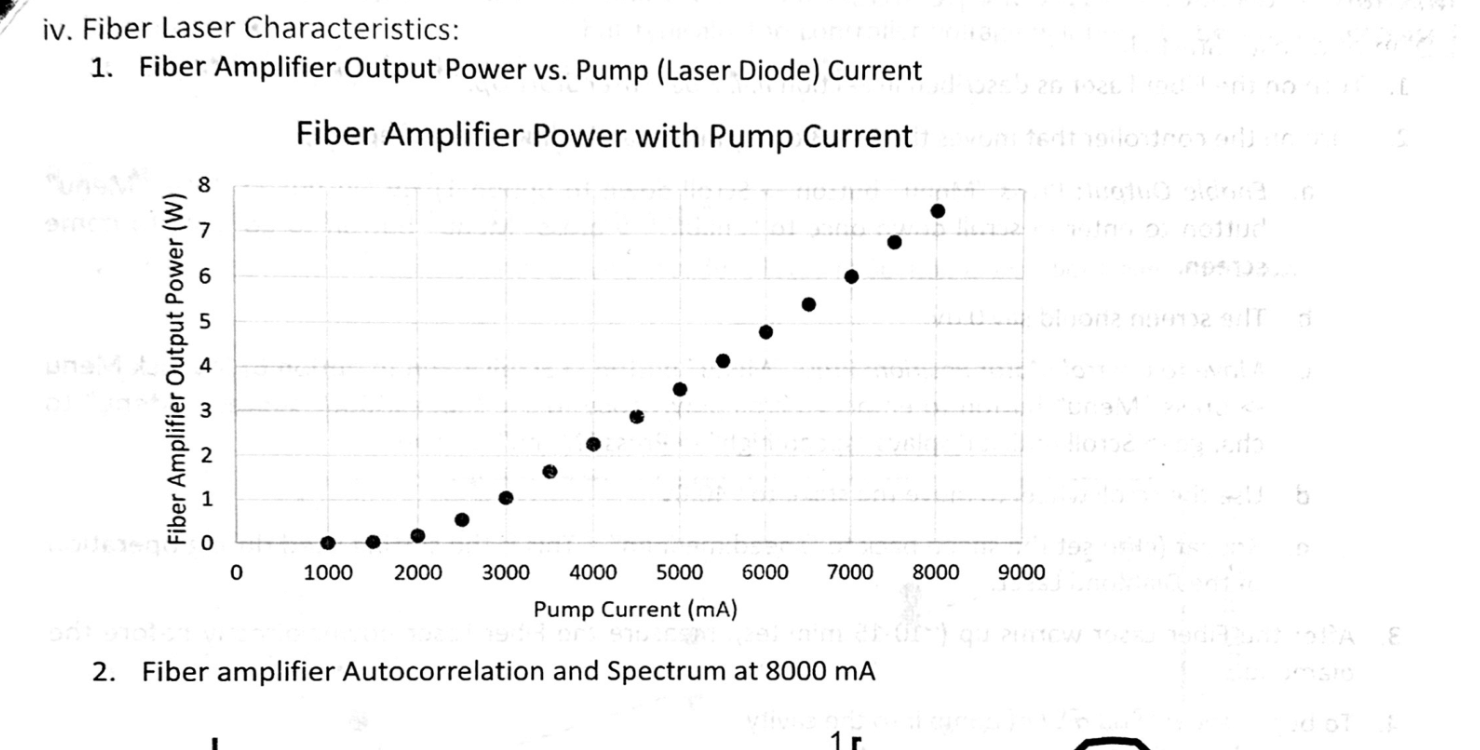
\includegraphics[width=0.8\linewidth]{fiber_power_curve.png}
  \caption{Fiber Amplifier Output Power vs.\ Pump Current.}
\end{figure}
\begin{figure}[ht]
  \centering
  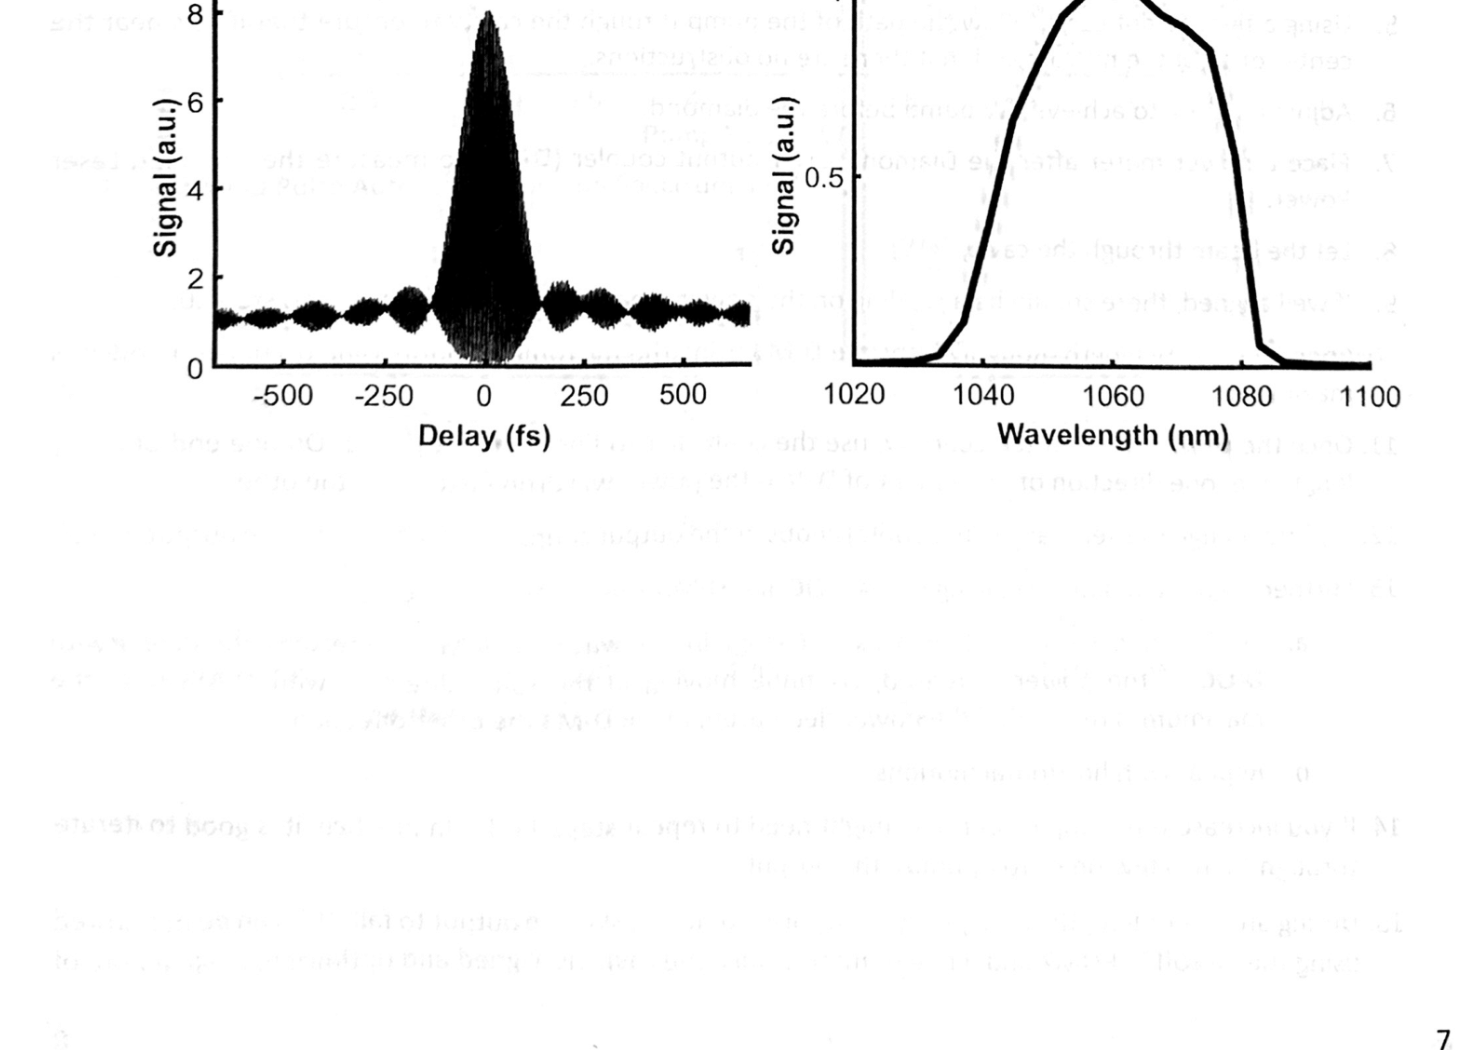
\includegraphics[width=0.8\linewidth]{fiber_autocorr_spectrum_8000mA.png}
  \caption{Autocorrelation and spectrum at 8000\,mA.}
\end{figure}

\section{Diamond Laser -- Typical Operation}

\subsection{Diamond Laser Start Up}
\begin{enumerate}
  \item Start the Fiber Laser as above.
  \item Turn on the D-M3 controller and enable HV output, set to 0.0\,V, set speed to high, move to 40.0\,V, then speed to medium.
  \item After 10--15\,minutes, measure fiber power before diamond.
  \item Allow $\sim$500\,mW pump into cavity.
  \item Trace beam on fluorescent card to check alignment.
  \item Adjust F-HWP2 to 4\,W pump before diamond.
  \item Place meter after D-OC for diamond output.
  \item Let beam through cavity (4\,W).
  \item Roughly translate D-M3 to lase and maximize.
  \item Fine-tune D-M3 and D-OC knobs.
  \item Walk beam vertically/horizontally with D-M3 and D-OC.
  \item Repeat if pump power changes.
  \item During experiments, monitor drift with D-POM2 and adjust.
\end{enumerate}

\subsection{Diamond Laser Shut Down}
\begin{enumerate}
  \item Turn off D-M3 controller.
  \item Follow Fiber Laser shut-down above.
\end{enumerate}

\subsection{Diamond Laser Characteristics}
\begin{figure}[ht]
  \centering
  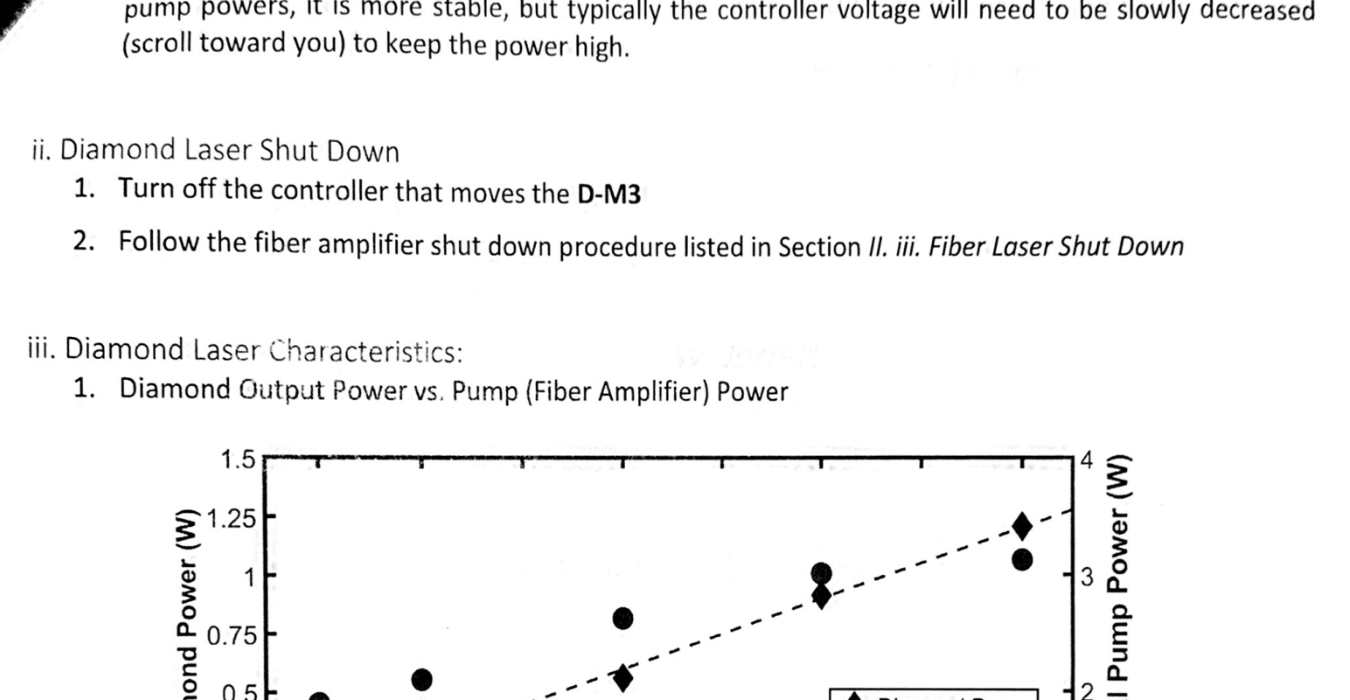
\includegraphics[width=0.8\linewidth]{diamond_power_curve.png}
  \caption{Diamond output power vs.\ pump power.}
\end{figure}
\begin{figure}[ht]
  \centering
  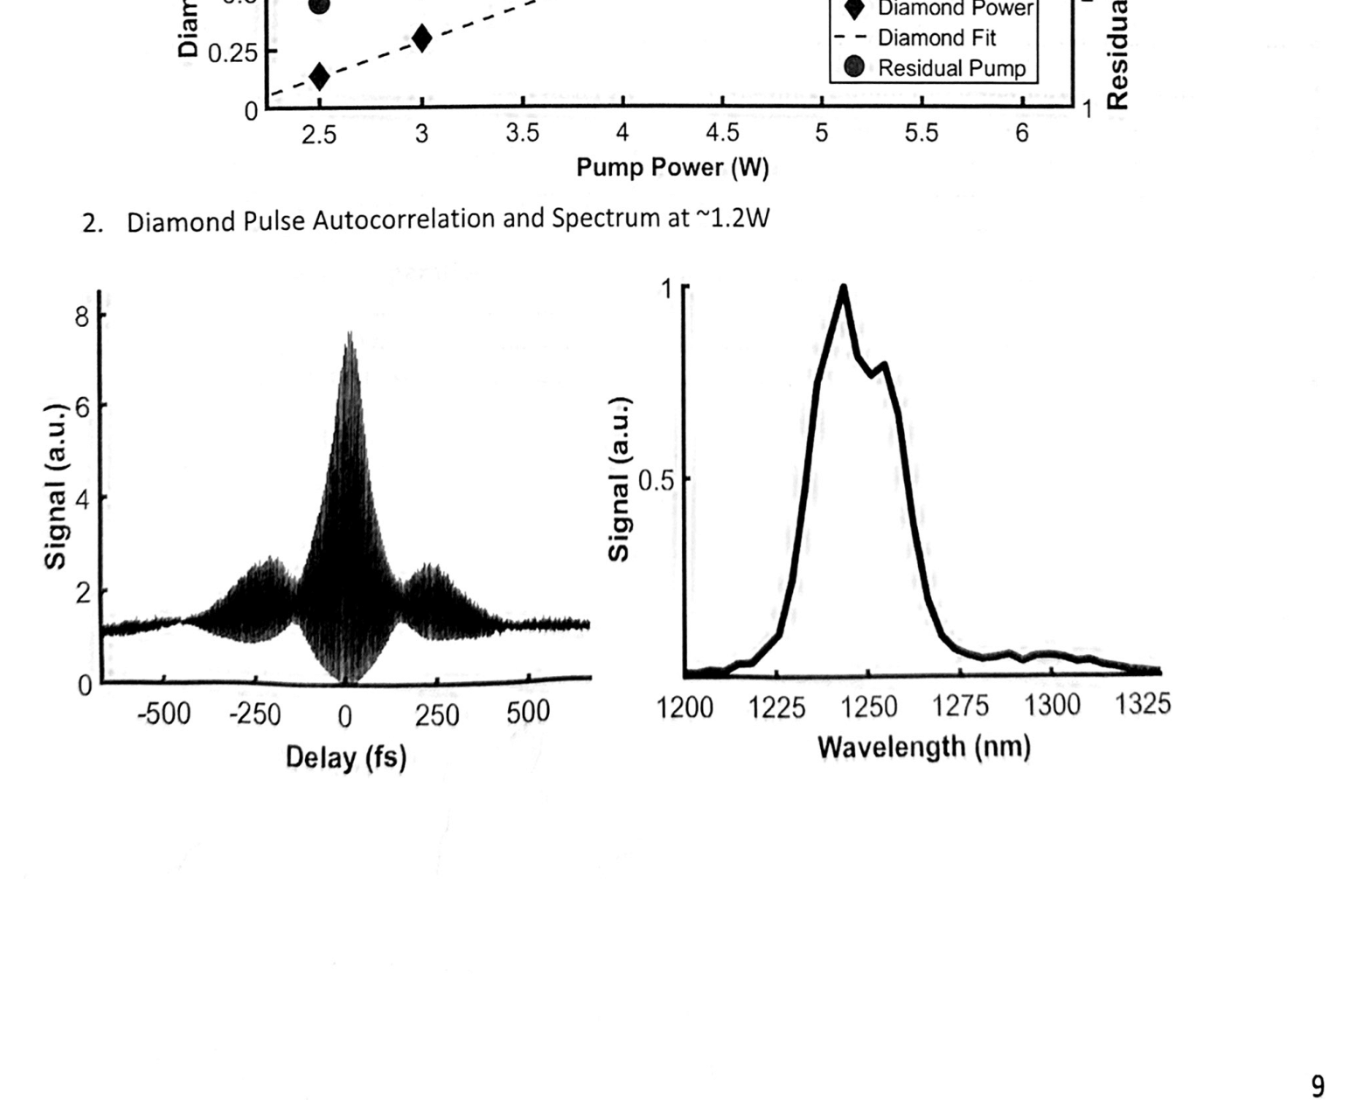
\includegraphics[width=0.8\linewidth]{diamond_autocorr_spectrum_1.2W.png}
  \caption{Autocorrelation and spectrum at ~1.2\,W.}
\end{figure}

\end{document}
